\chapter{Related work}
\label{chap:rel_work}
%TODO When done, fix this
This chapter discusses the relevant literature and state of the art for this thesis; the literature is grouped into x groups. In \autoref{section:routing_rel_work}, the routing algorithms for transport are discussed. Next, we examine the data models used in public transport (\autoref{section:data_model_rel_work}). Further, we look at existing ontologies for transportation in \autoref{section:ontologies_rel_work}.

\section{Transport Routing Algorithms }\label{section:routing_rel_work}
% include timeline image

\begin{figure}[H]
\resizebox{\textwidth}{!}{%
    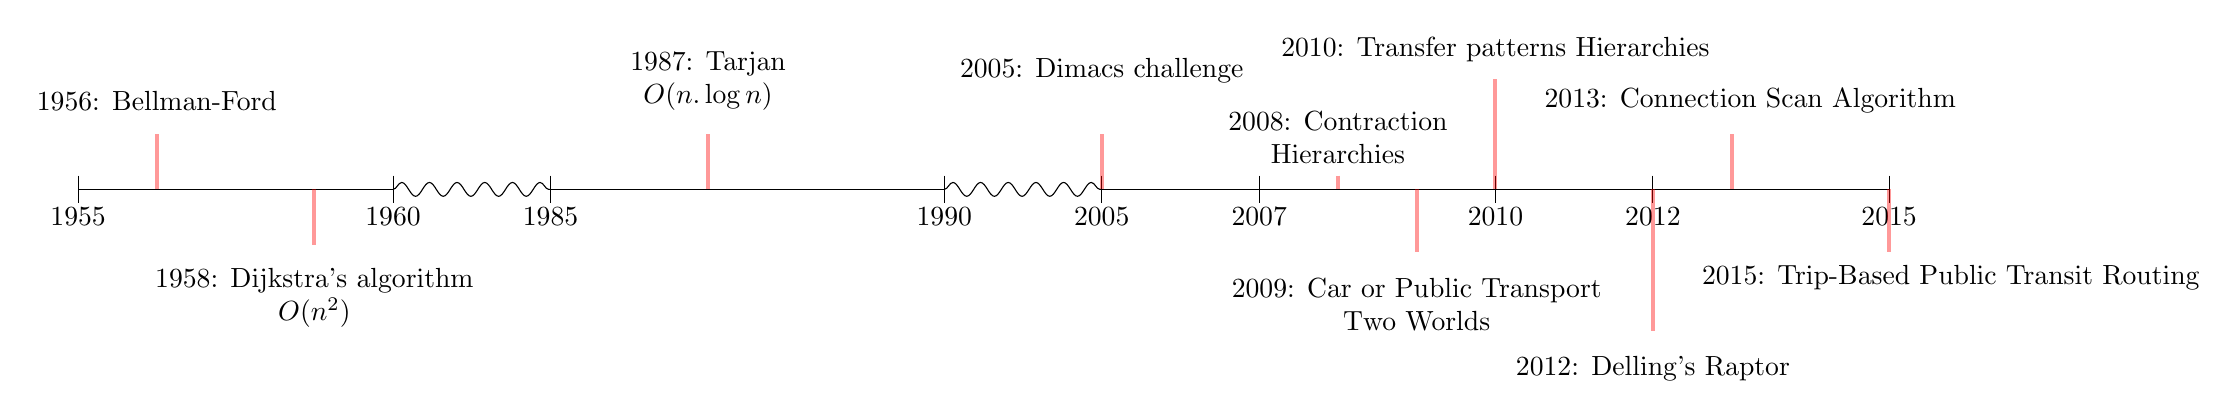
\begin{tikzpicture}
    % Draw a horizontal line
    \draw (0,0) -- (4,0);
    \draw (6,0) -- (11,0);
    \draw (13,0) -- (23,0);
    
    % draw vertical lines
    \foreach \x in {0,4,6,11,13,18,23,15,20}
    \draw (\x cm,5pt) -- (\x cm,-5pt);
    
    \foreach \x in {1,8,13,21}
    \draw[line width=0.5mm, red, opacity=0.4 ] (\x cm,20pt) -- (\x cm,0);
    
    \foreach \x in {3}
    \draw[line width=0.5mm, red, opacity=0.4 ] (\x cm,0) -- (\x cm,-20pt);
    
    % draw nodes to add events
    \draw (0,0) node[below=3pt] {1955};
    \draw (4,0) node[below=3pt] {1960};
    \draw (6,0) node[below=3pt] {1985};
    \draw (11,0) node[below=3pt] {1990};
    \draw (13,0) node[below=3pt] {2005};
    \draw (15,0) node[below=3pt] {2007};
    \draw (18,0) node[below=3pt] {2010};
    \draw (20,0) node[below=3pt] {2012};
    \draw (23,0) node[below=3pt] {2015};
    
    \draw (1,0) node[above=25pt] {1956: Bellman-Ford};
    
    \draw (3,0) node[below=25pt, align=center] {1958: Dijkstra’s algorithm\\ $O(n^2)$};
    
    \draw (8,0) node[above=25pt, align=center] {1987: Tarjan\\ $O(n.\log{n})$};
    
    \draw (13,0) node[above=35pt] {2005: Dimacs challenge};
    
    \draw (16,0) node[above=0.2cm, align=center] {2008: Contraction \\Hierarchies};
    \draw[line width=0.5mm, red, opacity=0.4 ] (16 cm,5pt) -- (16 cm,0);
    
    \draw (17,0) node[below=1cm, align=center] {2009: Car or Public Transport\\ Two Worlds};
    \draw[line width=0.5mm, red , opacity=0.4] (17 cm,0) -- (17 cm,-0.8cm);
    
    
    \draw (18,0) node[above=1.5cm] {2010: Transfer patterns Hierarchies};
    \draw[line width=0.5mm, red , opacity=0.4] (18 cm,1.4cm) -- (18 cm,0);
    
    \draw (20,0) node[below=2cm] {2012: Delling’s Raptor};
    \draw[line width=0.5mm, red, opacity=0.4] (20 cm,0) -- (20 cm,-1.8cm);
    
    \draw (21,0) node[above=32pt,right=-2.5 cm] {2013: Connection Scan Algorithm};

    \draw (23,0) node[below=32pt,right=-2.5 cm] {2015: Trip-Based Public Transit Routing};
    \draw[line width=0.5mm, red, opacity=0.4] (23 cm,0) -- (23 cm,-0.8cm);
    
    
    \draw[decoration={snake},decorate] (4,0) -- (6,0);
    \draw[decoration={snake},decorate] (11,0) -- (13,0);
    \end{tikzpicture}
    }
    \caption{Timeline describing the developments in route planning. The crossed parts represent}
    \label{fig:timeline}
\end{figure}

This section discusses the state of the art and history of public transport planning. Therefore, a tiny timeline (\autoref{fig:timeline}) was constructed to visualize some important milestones explained below. As seen in the timeline, most advances were made after 2009.

\subsection{Dijkstra}
% add some dijkstra algo workings, easy
The milestones between 1956 and 2008 did not apply to PT routing but focused on normal road networks. Among these milestones was the Dijkstra algorithm, published in 1958. This was the first big improvement but had a time complexity of $O(n^2)$. An improved version was proposed almost 30 years later, in 1987. It has a complexity of $O(n*\log(n))$ and is the version of the Dijkstra algorithm learnt at schools.% It works by initializing every node to $\infty$ except the source node, which is initialized to $0$. Then, every edge of the source node is visited. 
\subsection{Dimacs challenge}
No significant improvements for route planners were made until 2005. The road network of the US was published as part of the 9th Dimacs challenge \cite{noauthor_9th_2017}. A big deal for researchers, now they had an extensive dataset to test on. Many speedup techniques, mainly pruning techniques, were devised for the Dijkstra algorithms. But this was still inapplicable to \glsxtrshort{pt}.

\subsection{Car or Public Transport: Two Worlds}
In 2009 a paper, Car or Public Transport: Two Worlds \cite{bast_car_2009}, stated "There are two kinds of people: those who travel by car, and those who use public transport.". They argued that the worlds differed, although both problems could be represented as a directed graph. For PT, we must deal with timetable schedules besides this spatial information.

The article covers five big "tricks of the trade" for fast routing on transportation: Bidirectional search, exploiting hierarchy, graph contraction, goal direction and distance tables. It explains why the trick works on road networks but falls short on \glsxtrshort{pt}.

\subsubsection{Bidirectional search}
A simple approach to improve Dijkstra is to search from the source node but simultaneously do a backward search from the target node. This reduces the search space by half and can be quickly done for road networks since both nodes associated with the station are known. The idea is not very practical but is critical to implementing other speedup techniques.

For \glsxtrshort{pt}, this idea adds a lot of complexity since, in a time-expanded graph, we know the target station but not the target node. A solution is to do a backward set of all nodes associated with the end station.
\subsubsection{Exploiting hierarchy}
Roads have different levels of importance; think of motorways, national highways and minor roads. The simple routing heuristic exploits this hierarchy. When we are within a certain distance of the target and source node, we take all streets into account. In the other case, we use only high-level roads, reducing the total explored nodes. This comes with some loss of exactness.

However, this technique can be even slower in large municipal areas because the hierarchy is absent. The tram, metro and bus are equally important. A hierarchy begins to appear only when travelling long distances between cities. 
\subsubsection{Graph contraction}
For aesthetics, curved reads were replaced by multiple straight lines. This resulted in more edges and nodes, so researchers quickly reverted this. This is a contraction, and the resulting edge is called a shortcut. This even works in hierarchies because higher levels have junctions that would lead to lower levels. So, these junctions could be neglected and replaced by a shortcut. 

Similar to the previous problem, the hierarchy is absent. This technique does not work for \glsfmtshort{pt} in a large municipal area.
\subsubsection{Goal direction}
The Dijkstra algorithm is augmented with a heuristic, which leads to an algorithm like $ A*$. The performance is highly dependent on the heuristic chosen.

The problem is the lack of algorithms for local searches on \glsfmtshort{pt} networks, and this causes quadratic precomputations.
\subsubsection{Distance tables}
As the name suggests, this table contains the recalculated distances between all pairs of nodes in the graph. 

\subsection{Transfer patterns}
Transfer patterns are considered the first algorithm for PT that solves queries in an order of a few milliseconds and on a transport network with a poor structure. 

Transfer patterns describe a method using a journey planning algorithm to pre-calculate all the unique journeys for the entire graph \cite{bast_fast_2010} %wrong explanation of transfer graphs TODO FIX
. This means we can look up the schedule matching that journey when a real-time query comes in. In this case, the server can give fast query responses, but the pre-calculations can cause a computational burden. For example, the authors used a cluster of Opteron and Xeon-based 64-bit servers for their CPP implementation. Although the exact number of compute nodes is not mentioned in the paper \cite{bast_fast_2010}. They do mention the needed core hours, arround 3000, so if run on a single-core this would take about 4 months to finish.  


% TODO uitleggen transfer paterns
A simple algorithm for transfer patterns illustrates the key ideas and consists of 3 parts but has quadratic precomputation complexity. A more optimized algorithm is described in the paper \cite{bast_fast_2010}.
\subsubsection{Graph}
The algorithm works on a time-expanded graph with three kinds of nodes: a departure node, an arrival node and a transfer node. Each node carries the time and the station it belongs to. Like in \autoref{fig:transferel}.
\begin{figure}[H]
\begin{minipage}{.45\textwidth}

\centering
\resizebox{0.5\linewidth}{!}{%
    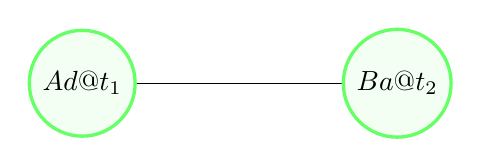
\begin{tikzpicture}[
roundnode/.style={circle, draw=green!60, fill=green!5, very thick, minimum size=8mm},
]
    
    \draw (0,0) -- (4,0);
    
    \draw (4,0) node[align=center,roundnode] {$Ba@t_2$};

    \draw (0,0) node[align=center,roundnode] {$Ad@t_1$};
    
    \end{tikzpicture}
%
}%
    \caption{An elementary connection betweens stations A and B, d stands for departure and a for arrival, $@t_i$ denotes the time the vehicle departs, arrives are waits (transfer)}
    \label{fig:transferel}

\end{minipage}\hspace{.1\textwidth}
\begin{minipage}{.45\textwidth}
\centering
\resizebox{0.5\linewidth}{!}{%
    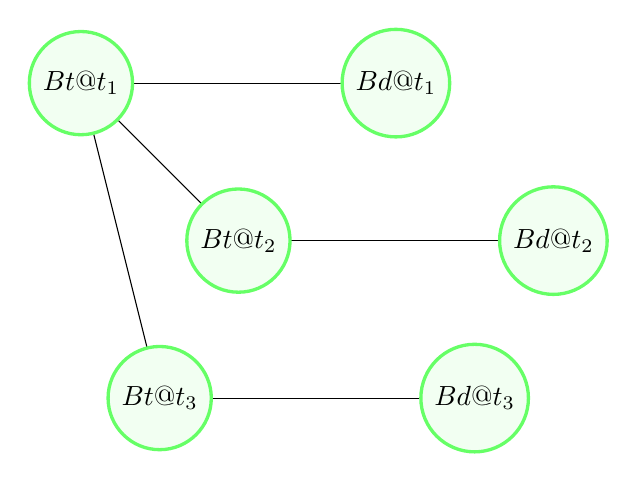
\begin{tikzpicture}[
roundnode/.style={circle, draw=green!60, fill=green!5, very thick, minimum size=8mm},
]
    
    \draw (0,0) -- (4,0);
    \draw (0,0) -- (2,-2);
    \draw (0,0) -- (1,-4);
    \draw (1,-4) -- (5,-4);
    \draw (2,-2) -- (6,-2);
    
    \draw (0,0) node[align=center,roundnode] {$Bt@t_1$};

    \draw (4,0) node[align=center,roundnode] {$Bd@t_1$};


    
    \draw (2,-2) node[align=center,roundnode] {$Bt@t_2$};

    \draw (6,-2) node[align=center,roundnode] {$Bd@t_2$};

    \draw (1,-4) node[align=center,roundnode] {$Bt@t_3$};

    \draw (5,-4) node[align=center,roundnode] {$Bd@t_3$};
    \end{tikzpicture}
%
}%
    \caption{An transfer, with an waiting chain}
    \label{fig:transferpatterntransfer}

\end{minipage}
\end{figure}
\subsubsection{Fast direct-connections queries}
This part is only for direct connections, meaning a maximal path in the graph without transfer nodes.

\begin{enumerate}
    \item Precompute all maximal paths in the graph without transfer nodes. Group them in lines that share the same sequence of stations. This creates an ordered timetable for a particular line.
    \item Precompute for each station the sorted list of lines in which the station occurs and its position(s) on the line. This creates a lookup table, which can be used to find timetables of lines stations share.
    \item To answer a direct connection query, use the precomputed sorted list of the departure and arrival stations. See if they share a line with the departure station, which has a lower position than the arrival station. Using the timetables of the found lines, determine the earliest arrival time.
\end{enumerate}
\subsubsection{Transfer patterns precomputation}

\subsubsection{Query graph construction and evaluation}
\subsubsection{scalable transfer patterns}
The paper of Scalable transfer patterns \cite{bast_scalable_2015} identifies two criteria (the space consumption of the precomputed auxiliary data is large and the preprocessing time is huge) in which transfer patterns are lacking. Furthermore the scalabilty of transfer patterns are addressed by introducing a new scheme based on clustering the network for Transfer Patterns precomputation and query graph construction that allows interactive query times for huge transit networks with manageable preprocessing times and space consumption. 
\subsection{\glsfmtfull{csa}}
\subsection{Trip-based public transit routing}

\subsection{\glsfmtfull{raptor}}
RAPTOR is a graph-based algorithm that solves queries in rounds. Round K computes the fastest way of getting to every stop with at most k - 1 transfers or k trips.

\begin{enumerate}
    \item Each node gets a multilabel. $(\tau_0,...,\tau_k)$ with $\tau_i$ representing the earliest arrival time in $i$ trips. We init all arrival times in each label with $\infty$. Except for the departing node, where $\tau_0$ is set to the depart time of our search criteria.
    \item For each round $k$ our goal is to compute $\tau_k$. This happens in three stages:\begin{enumerate}
        \item Set the earliest arrival time k ($\tau_k$) to that of iets predescor ($\tau_{k-1}$). This is an upper bound since we are not interested in slower stop times than the previous round.
        \item We iterate over the routes. We calculate the earliest trip we can take for each stop $p$ on the route $r$. This does not always exist. We search stops along the route $r$ with the earliest trip $t$. This means we can hop on the route $r'$ in $p$. For subsequent stops in $r'$, we can update $\tau_k$ according to the found trip $t$.
        \item Finally, footpaths are considered. We check if $\tau_k$ can be improved by using a footpath between two stops. 
    \end{enumerate}
\end{enumerate}


\begin{figure}[H]
\centering
\resizebox{\textwidth}{!}{%
    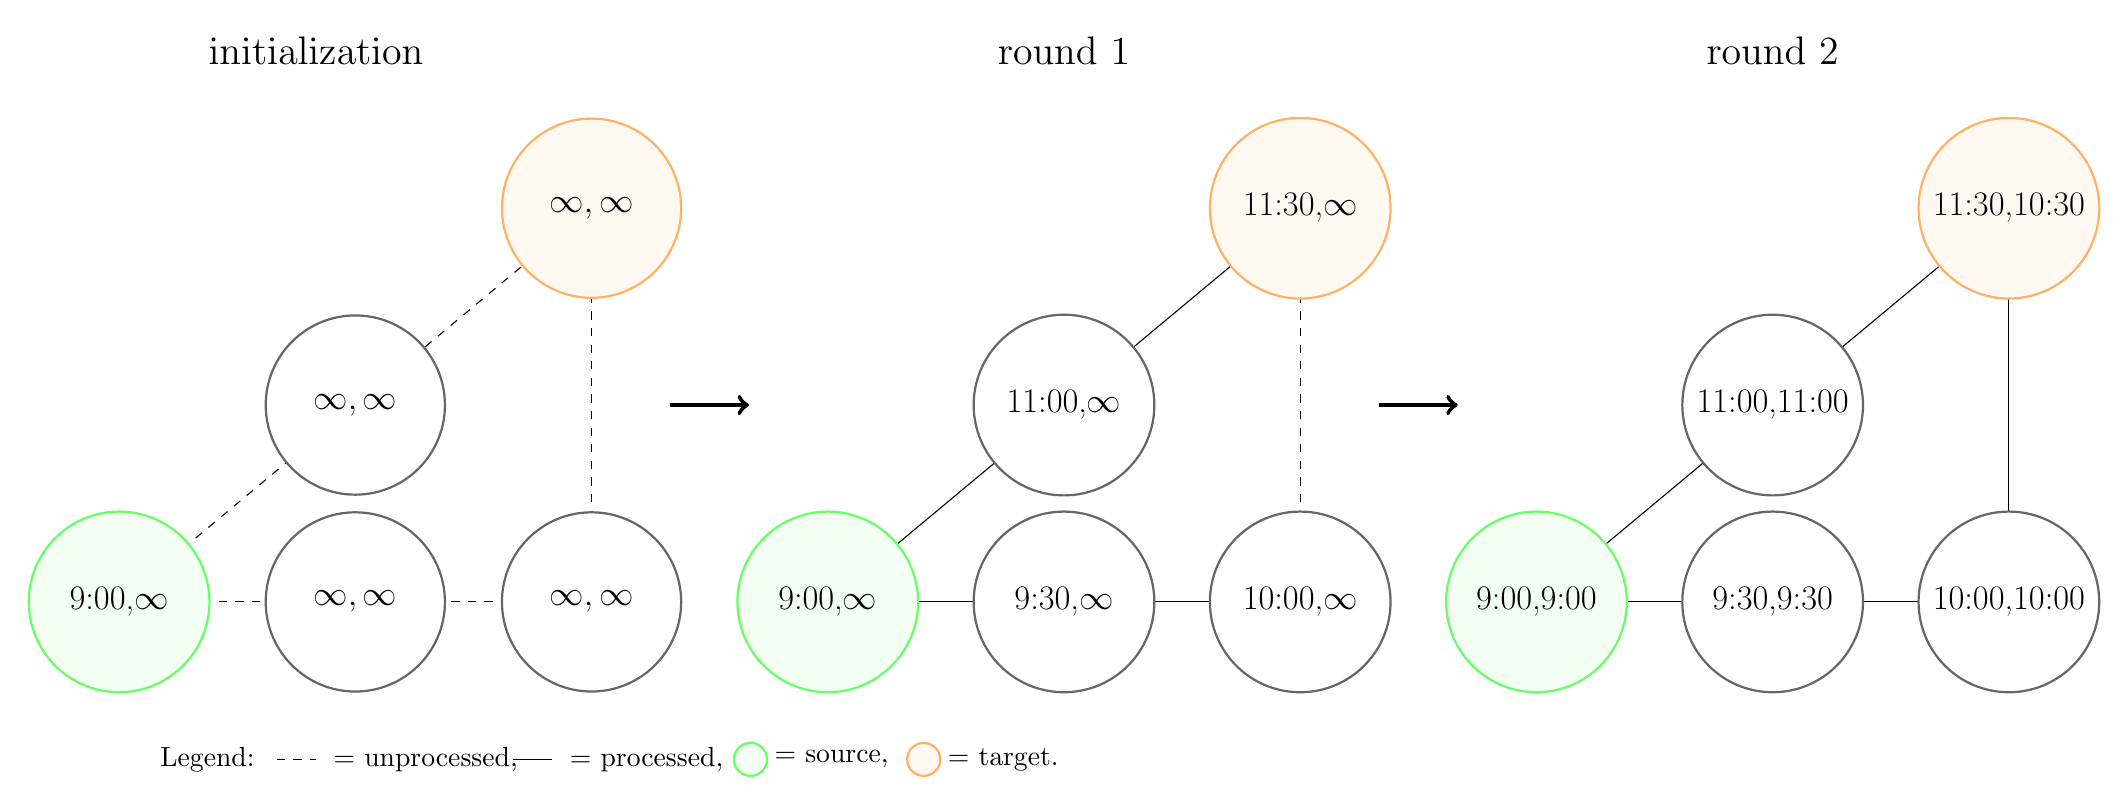
\begin{tikzpicture}[
roundnode/.style={circle, thick, minimum size=7mm, text width=3.5cm,align = center,scale=0.6,font=\huge},
green/.style={draw=green!60, fill=green!5},
orange/.style={draw=orange!60, fill=orange!5},
white/.style={draw=black!60, fill=white},
]
    \draw (0.4,-2) node[right=0] {Legend:};
    \draw [dashed](2,-2) -- (2.5,-2);
    \draw (2.6,-2) node[right=0] {= unprocessed,};
    \draw [](5,-2) -- (5.5,-2);
    \draw (5.6,-2) node[right=0] {= processed,};
    \draw (7.8,-2) node[roundnode,text width=0.4cm,green,right=0] {};
    \draw (8.2,-2) node[right=0] {= source,};
    \draw (10,-2) node[roundnode,text width=0.4cm,orange,right=0] {};
    \draw (10.4,-2) node[right=0] {= target.};
    
    \draw [dashed](0,0) -- (6,0);
    \draw [](9,0) -- (15,0);
    \draw [](18,0) -- (24,0);
    

    \draw [dashed](6,0) -- (6,5);
    \draw [dashed](15,0) -- (15,5);
    \draw [](24,0) -- (24,5);
    

    \draw [dashed](0,0) -- (6,5);
    \draw [](9,0) -- (15,5);
    \draw [](18,0) -- (24,5);
    
    \draw[->, ultra thick] (7,2.5) -- (8,2.5);
    \draw[->, ultra thick] (16,2.5) -- (17,2.5);
    
    \draw (0,0) node[roundnode,green] {9:00,$\infty$};
    \draw (3,0) node[roundnode,white] {$\infty,\infty$};
    \draw (6,0) node[roundnode,white] {$\infty,\infty$};
    \draw (3,2.5) node[roundnode,white] {$\infty,\infty$};
    \draw (6,5) node[roundnode,orange] {$\infty,\infty$};

    
    \draw (9,0) node[roundnode,green] {9:00,$\infty$};
    \draw (12,0) node[roundnode,white] {9:30,$\infty$};
    \draw (15,0) node[roundnode,white] {10:00,$\infty$};
    \draw (12,2.5) node[roundnode,white] {11:00,$\infty$};
    \draw (15,5) node[roundnode,orange] {11:30,$\infty$};

    
    \draw (18,0) node[roundnode,green] {9:00,9:00};
    \draw (21,0) node[roundnode,white] {9:30,9:30};
    \draw (24,0) node[roundnode,white] {10:00,10:00};
    \draw (21,2.5) node[roundnode,white] {11:00,11:00};
    \draw (24,5) node[roundnode,orange] {11:30,10:30};

    \draw (2.5,7) node[font=\Large] {initialization};
    \draw (12,7) node[font=\Large] {round 1};
    \draw (21,7) node[font=\Large] {round 2};
    \end{tikzpicture}
%
}%
    \caption{A small example using raptor, two rounds are show}
    \label{fig:raptor_example}
\end{figure}

\subsubsection{Hyper partitioning}
Hyper partitioning is a preprocessing-based acceleration technique for computing bi-criteria Pareto-optimal journeys in public transit networks, based on the well-known RAPTOR algorithm \cite{delling_round-based_2015}.
\subsubsection{unrestricted footprints}
% TODO WIP
This work presents a new algorithm that uses trips (vehicles) and the transfers between them as its fundamental building blocks. Unlike existing algorithms, it does not assign labels to stops. Instead, trips are labelled with the stops at which they are boarded.
\section{Data Models For public transport}\label{section:data_model_rel_work}

\subsection{What is a data model }
% TODO CHECK AND REWRITE 
% FROM https://cedar.princeton.edu/understanding-data/what-data-model
A data model organizes data elements and standardizes how the data elements relate to one another. Since data elements document real-life people, places, and things and the events between them, the data model represents reality. For example, a house has many windows, or a cat has two eyes.

Data models are often used to communicate between the business people defining the requirements for a computer system and the technical people defining the design in response to those requirements. They are utilized to show the data needed and created by business processes.
 
A data model explicitly determines the structure of data. Data models are specified in a data modelling notation, which is often graphical in form.]
A data model can sometimes be called a data structure, especially in programming languages. Function models often complement data models.
\subsection{\glsfmtfull{gtfs}}
\glsfmtfull{gtfs} defines a common format for public transportation schedules and associated geographic information. "feeds" let public transit agencies publish their transit data. The developer can then write applications.

GTFS
"Downstream" 
+ widely used format for distributing timetables to third
  parties
- not all fare products and schemes are supported
- custom software needed for interpretation 
+ dataset available of NMBS

\subsubsection{\glsfmtshort{gtfs} feed}
A feed is a zip file containing CSV files but typically has the .txt extension. Some essential files include stops.txt, routes.txt, and trips.txt.


\subsection{\glsfmtfull{netex}}
The NeTEx defines a standard for exchanging public transport passenger information data in XML format. The functional
scope of NeTEx is divided into three parts, each covering a functional subset of the CEN Transmodel conceptual
model for Public Transport Information, [T1], [T2], [T3].
Part 1 [N1]] describes the fixed Network (stops, routes, lines, etc.); Part 2 [N2] is mainly focused on Timetables and
Part 3 [N3] covers Fare data (and is the main subject of this paper). All three parts use the same framework of reusable
components, versioning mechanism, validity conditions, and support to allow the unique identification of data elements
in a global context, etc., defined in Part 1. NeTEx also includes container elements called "VERSION FRAMES"
to group data into coherent sets for efficient exchange.
NeTEx deliverables comprise (i) a CEN Specification document (in three parts), (ii) a data model in the standard UML
modelling language [U1] and (iii) an accompanying XML schema providing a formal electronic description that can
be used by data processing software.

Data in NeTEx format is encoded as XML documents that must conform exactly to the schema – standard XML validator tools can check conformance automatically. The schema can also be used to create bindings for different
programming languages, automating part of the implementation process for creating software that supports NeTEx
formats. 

NeTEx (Network Timetable Exchange)
"upstream"

Based on the transmodel ontology, Identification of Fixed Objects in Public Transport or IFOPT (as of part 2) and SIRI.

Part one describes the topology format or the fixed Network (stops, routes,lines...)

Part two defines the scheduled timetables exchange format

Part three defines fare exchange format

NeTEx documents are in xml format and must cohere to shema's.
+ All mass public transport modes supported in part one
- Content is directly derived from transmodel
- only a subset of transmodel is covered
+ CEN Technical Specification
+ dataset available of NMBS
+ Entire data set can be one document
- Extra functionalities can add unnecessary complexity
+ Can be checked using xml validator


\subsubsection{NETEX profiles}
\subsection{Transmodel}
\section{Semantic Web and the role of Ontologies}\label{section:ontologies_rel_work}
\subsection{Semantic Web}
The semantic web can be seen as an extension of the current web and is a vision of Tim Berners-Lee, where web documents not only describe how to render data visually. The data is also annotated with terms to express how it should be interpreted. So, web documents also capture the meaning of the information.

Linked data- structured data that is interlinked with other data- is the basis of the Semantic Web. It builds upon existing protocols such as HTTP, RDF, and URIs.

\begin{itemize}
    \item Use URIs as names for things

    \item Use HTTP URIs so that people can look up those names.

    \item When someone looks up a URI, provide useful information using the standards (RDF*, SPARQL)

    \item Include links to other URIs. so that they can discover more things.

\end{itemize}

Besides linked data, Sir Tim Berners-Lee also proposes a classification of data sources. It is a five-star deployment scheme for open data \cite{noauthor_5-star_nodate}.

\begin{enumerate}
    \item $\star$: Make your stuff available on the web (whatever format) under an open license
    \item $\star\star$ make it available as structured data (e.g., Excel instead of image scan of a table)
    \item $\star\star\star$ make it available in a non-proprietary open format (e.g., CSV instead of Excel)
    \item $\star\star\star\star$: use URIs to denote things so that people can point at your stuff
    \item $\star\star\star\star\star$:link your data to other data to provide context.
\end{enumerate}

\subsection{Resource Description Framework}
\subsection{JSON-LD}
%\subsection{RML}

\subsection{Ontologies}
The best definition of an ontology states: "An ontology is an explicit specification of a conceptualization" \cite{gruber_translation_1993}. Many ontologies exist, from basic to formal ontologies specified in highly expressive logic. In this thesis, we mainly use formal ontologies.

These ontologies play an essential role in the semantic web. 

A small study was conducted to find an ontology that best suited our needs. Many of the studied ontologies for transport are focused on specific use cases, for example, urban freight \cite{bouhana_ontology-based_2015}. They do not have a broad domain. 

Ontologies of Wayfinding: a Traveler’s Perspectiv (https://doi.org/10.1023/A:1014563113112), 2002
describes two ontologies of “wayfinding” with multiple transportation modes in an urban area based on two perspectives: the traveler and the public transportation system.
- Properties, relations and axioms not defined. Focus on concepts only.
- focussed on an urban area

An Ontology-based Public Transport Query System (DOI: 10.1109/SKG.2005.41)
- server side 

 A public transportation ontology to support user travel planning (https://doi.org/10.1109/RCIS.2010.5507372), 2010
Domain ontology with OWL 1.0. Validation done using 
+ Designed for use with a planning tool
+ Can be used country wide
+ journey patterns (similar to raptor)
+ Footpaths supported in form of infrastructure points
- ontology not directly available, snippets in pdf
- planning server side

\subsection{x}
A relatively old ontology designed to use with a user planning tool based on journey patterns \cite{5507372} was found and could support RAPTOR. Interestingly, they implemented a mobile application to plan tourist bus routes, but it relied on server-side queries. Other downsides are that there is no multi-modal support (only transport by bus) and no multi-operator support. The ontology was not directly available from the authors.

Using the survey of transportation ontologies \cite{katsumi_ontologies_2018}, we only identify three ontologies that support journey patterns—two of which focus on city logistics and urban systems, which are different domains. The last ontology (Transportation ontology for content personalization) applies to PT, but the ontology is not directly available.

\subsection{Transmodel ontology}
European directives require every PT agent to be compatible with Transmodel, so an ontology aligned with Transmodel is interesting. Further, the Transmodel ontology supports journey patterns. However, the ontology could be too broad, which leads to several potential problems. For example, it can make it hard to find relevant information, as the ontology may contain too many concepts and relationships that are not relevant. Furthermore, as the ontology may not be compatible with other ontologies used in those sources, integration from different sources can also be challenging.

\subsection{OSLO Mobiliteit: Dienstregeling en Planning}
The last ontology we looked at is the "OSLO Mobiliteit - Dienstregeling en Planning" \cite{noauthor_oslo_2023} ontology. The ontology is developed by Open Standaarden voor Linkende Organisaties (OSLO), a department of Data Flanders. It has been based on the EPIP profile of NETEX. NETEX is based directly on Transmodel, so the ontology has some similarities with the Transmodel ontology but is less broad than the Transmodel ontology.

 Het applicatieprofiel OSLO Mobiliteit – Dienstregeling en Planning: Tijdstabellen beschrijft hoe de termen uit het overeenkomstig vocabularium moeten worden gebruikt om de netwerktopologie en dienstregeling van een openbaar vervoersnetwerk te beschrijven.

De standaard is gebaseerd op het EPIP-profiel op NETEX.

Use-cases voor deze standaard zijn: routeplanning, cartografie (netplannen), dienstregeling en het opzoeken van haltes/lijnen.

Openbaar vervoer wordt typisch aangeboden onder de vorm van Lijnen, die bv op basis van de transportmodus (trein, tram, bus… ) gegroepeerd kunnen worden en deel uitmaken van een Netwerk. Deze Lijnen volgen bepaalde Routes op het terrein, het model laat toe de richting en de geometrie van deze Routes te beschrijven dmv Routepunten en verbindingen daartussen, de Routelinks.

Een ander deel van het model beschrijft de dienstverlening die door de Lijnen wordt geboden: de plaatsen waar gestopt wordt en de tijdstippen waarop daar wordt gestopt.

Een Lijn volgt een zgn Ritpatroon, ttz de opeenvolging van Punten die door de Lijn worden aangedaan. De specialisatie daarvan, een Dienstpatroon, beschrijft de opeenvolging van Punten waar werkelijk gestopt wordt. Dit zijn de zgn GeplandeStoppunten: plaatsen waar passagiers kunnen op- of afstappen. Deze logische haltes kunnen gelinkt worden met fysieke haltes (klasse Stopplaats) die apart beschreven worden in het applicatieprofiel OSLO Mobiliteit – Dienstregeling en Planning: Stopplaatsen.

Voor elk punt dat wordt aangedaan door een Lijn of waar voor passagiers wordt gestopt kunnen Doorkomsttijden worden opgegeven. Deze kunnen gegroepeerd worden per halte en vormen dan de typische tijdstabellen die men daar aantreft. Ze kunnen ook geordend worden volgens het Ritpatroon van een Lijn en beschrijven dan een individuele Dienstrit met de Doorkomsttijden aan de haltes.

Een specifieke Dienstrit wordt niet noodzakelijk dagelijks uitgevoerd, het kan zijn dat hij beperkt is tot bepaalde Dagtypes, bv enkel op weekdagen. Het model laat toe om deze Dagtypes te beschrijven en te koppelen aan werkelijke datums (OperationeleDagen) en periodes (OperationelePeriodes) om zo te komen tot een volledige Dienstkalender.

Tot slot vermelden we nog ondersteunende klassen bv om de partijen die het vervoer aanbieden of uitvoeren (resp de Autoriteit en de Operator) aan te duiden of om Voertuigtypes en hun Passagierscapaciteit te beschrijven of een klasse die routeplanning ondersteunt (Dienstritverbinding). 
\begin{landscape}
\begin{table}[]
\centering
\begin{tabular}{|l|l|l|l|l|l|l|}
\hline
\textbf{Ontology} &
  \textbf{\begin{tabular}[c]{@{}l@{}}Journey\\ patterns?\end{tabular}} &
  \textbf{\begin{tabular}[c]{@{}l@{}}Multi-\\ modal?\end{tabular}} &
  \textbf{\begin{tabular}[c]{@{}l@{}}Multi-\\ operator?\end{tabular}} &
  \textbf{\begin{tabular}[c]{@{}l@{}}Designed for use\\  with routeplanners\end{tabular}} &
  \textbf{\begin{tabular}[c]{@{}l@{}}directly available\\  for reuse?\end{tabular}} &
  \textbf{DOI} \\ \hline
\begin{tabular}[c]{@{}l@{}}Intoducing the public transport\\ domain to the web of data\end{tabular} &
  yes &
  yes &
  yes &
  yes &
  no &
  10.1007/978-3-319-11746-1\_38a \\ \hline
iCity Ontology &
  yes &
  no &
  no &
  no, urban systems &
  yes, GitHub &
  w3id.org/icity/iCityOntology\_v1\_Report.pdf \\ \hline
Genclon &
  yes &
  no &
  no &
  no, city logistics &
  no &
  10.1016/j.eswa.2012.03.068 \\ \hline
\begin{tabular}[c]{@{}l@{}}Transportation ontology\\ for content personalization\end{tabular} &
  yes &
  yes &
  yes &
  yes &
  no &
  10.1016/j.eswa.2012.12.028 \\ \hline
Transmodel ontology &
  yes &
  yes &
  yes &
  yes &
  yes, GitHub &
  10.3233/SW-210451 \\ \hline
OSLO Ontology &
  yes &
  yes &
  yes &
  yes &
  yes &
  / \\ \hline
\end{tabular}
\caption{}
\label{tab:my-table}
\end{table}
\end{landscape}
\cite{noauthor_otp_2023}.